\documentclass[a4paper,11pt,makeidx]{report} % Font size

\usepackage{makeidx}
\usepackage{color}
\usepackage{listings}
\usepackage{graphicx}
\usepackage{hyperref}
\usepackage[nohyphen]{underscore}
\usepackage{url}

\hypersetup{colorlinks=true}

\bibliographystyle{abstract}

%%% AH Macros
\long\def\comment#1{}%
\def\pipkw{\tt\bf\color{blue}}%
\def\PIPKW#1{{\tt #1}}%
\def\pipterm#1{{\pipkw #1}\index{PiP Term!#1}}%
\def\PIPID{\pipterm{PIPID}}%
\def\pipfunc#1{{\pipkw #1}\index{PiP Function!#1}}%
\def\pipstruct#1{{\pipkw #1}\index{PiP Type!#1}}%
\def\pipcmd#1{{\pipkw #1}\index{PiP Command!#1}}%
\def\pipenv#1{{\pipkw #1}\index{PiP Environment Variable!#1}}%
\def\pipdef#1{{\pipkw #1}\index{PiP Define Symbol!#1}}%

\def\linuxfunc#1{{\tt #1}\index{Linux Function!#1}}%
\def\linuxcomm#1{{\tt #1}\index{Linux Command!#1}}%
\def\linuxenv#1{{\tt #1}\index{Linux Environment Variable!#1}}%
\def\linuxdef#1{{\tt #1}\index{Linux Define Symbol!#1}}%
\def\linuxvar#1{{\tt #1}\index{Linux Variable!#1}}%

\def\term#1{#1\index{#1}}%
\def\mpi#1{{\tt #1}\index{MPI!#1}}%
\def\NULL{\tt NULL}%
\def\PIE{PIE\index{PIE}}%
\def\PIC{PIC\index{PIC}}%

\def\arch#1{{\tt #1}\index{CPU Architecture!#1}}
\def\AMD{{\tt x86\_64}}%
\def\INTEL{{\tt x86\_32}}%
\def\ARM{{\tt AArch64}}%

\def\option#1{$\langle$#1$\rangle$}%

\lstloadlanguages{C,csh}

\lstset{basicstyle=\small\tt, numberbychapter=true, showstringspaces=false,
  emph={pip_get_pipid, pip_get_ntasks,
    pip_init, pip_fin,
    pip_spawn, pip_wait, pip_wait_any, pip_trywait, pip_trywait_any, 
    pip_task_spawn, pip_spawn_program_t,
    pip_spawn_from_func, pip_spawn_from_main,
    pip_spawn_hook, pip_spawn_hook_t,
    pip_named_export, pip_named_import, pip_exit, 
    pip_barrier_init, pip_barrier_wait, pip_barrier_fin,
    pip_barrier_t, pip_gettime, pip_gettid,
    pip_glibc_lock, pip_glibc_unlock,
    PIP_PIPID_ROOT, PIP_PIPID_ANY, PIP_PIPID_MYSELF, 
    PIP_CPUCORE_ASIS, PIP_CPU_CORE_ABS,
    PIP_MODE_PTHREAD, PIP_MODE_PROCESS,
    PIP_STOP_ON_START, PIP_GDB_SIGNALS, PIP_SHOW_MAPS,
    PIP_SHOW_PIPS, PIP_GDB_PATH, PIP_GDB_COMMAND,
    pip-exec, pipcc, pipfc, pip-mode, printpipmode, pip-gdb}, 
  emphstyle={\pipkw}, texcl=true, escapeinside={<(}{)>}}


\lstdefinestyle{program}{numbers=none, numberstyle=\tiny, numbersep=5pt, frame=tb, language=C}
\lstdefinestyle{example}{numbers=none, numberstyle=\tiny, numbersep=5pt, language=, frame=tRBl}
%%\lstdefinestyle{define}{frame=single, language=csh}

\title{Great Experiences with PiP (Proecss-in-Process)} % Book title
\author{Atsushi Hori} % Author

%--------------------------------------------------------------------------------
\makeindex

\begin{document}
%%\maketitle
\begin{titlepage}
	\centering
	
\includegraphics[width=0.25\textwidth]{Figs/PiP-logo.pdf}
        \par\vspace{3cm}
	{\huge\bfseries Great Experiences with PiP (Proecss-in-Process)\par}
	\vspace{9cm}
	{\Large Atsushi Hori\par}
	\vfill
% Bottom of the page
	{\Large \today\par}
\end{titlepage}

\newpage % Make sure the following content is on a new page

%----------------------------------------------------------------------------------------
%	TABLE OF CONTENTS
%----------------------------------------------------------------------------------------

\chapter*{Preface}

I retired from my work from April 2022. Since then, I wrote this PiP
tutorial. At the same time, I am maintaining PiP library
(\url{https://github.com/procinproc}).



Since PiP provides a new execution model not yet widely accepted, I am
not confident with adapting PiP with the newer Glibc (currently
supporting the Glibc attached with CentOS/Redhat 7 and 8). This is
because the PiP implementation is heavily depending on the niches of
Glibc. 


\tableofcontents % Prints the table of contents
\listoffigures
\listoftables
\lstlistoflistings

\chapter*{Acknowledgment}

The predecessor of PiP is PVAS (Partitioned Virtual Address Space)
developed by Akio Shimada. The idea of using PIE was his idea. Pavan
Balaji has a great insight and he saw through the possibilities of
PVAS at the first time Akio and I had a meeting with him. He also gave
me some great ideas when developing PiP. The name of PiP was his
recommendation. Min Si devoted her lots of time to help me writing PiP
papers. Kaiming Ouyang wrote great papers to improve MPICH performance
by using 
PiP. Yutaka Ishikawa allowed me to devote most of my time for
developing PiP.  Balazs Gerofi also gave me some useful comments on
PiP. Noriyuki Soda helped me a lot while developing PiP and he developed
the Github actions for testing PiP.

Finally, I thank to my wife, Fusa Hori, allowing me to devote my time
for writing this book.


\chapter*{Introduction}

\section{Introduction}

blablabla
\label{sec:intro}

\chapter{PiP Basics}\label{chap:basics}

Let me start describing the PiP basics for those who are not
familiar with PiP; 1) how to run a PiP program, 2) How to write a PiP
program, and 3) usage of PiP commands. The explanations in this
chapter does not go into details. For more details, refer to the 
Chapter~\ref{chap:advanced} and/or the other documents (man pages and
PDF). 


\section{PiP Tasks}

This section will explain how PiP tasks are created simply and how
they operate differently from processes (made using \term{MPI}) and
threads (created using \term{OpenMP}).

\subsection{\PIPKW{pipcc} and \PIPKW{pip-exec} Commands}
\label{sec:pipcc-exec}

The first example is  the well-known C program ``hello world'' listed
below; 

\lstinputlisting[style=program, caption={Hello World
    ({\tt hello.c})},label=prg:hello] {tasks/examples/hello.c}

As you can see, this program is a perfect match for a standard C
program. If the \pipcmd{pipcc} command was used to compile the
program, it can be run as a standard C program or as a PiP task by
using the \pipcmd{pip-exec} command.

\lstinputlisting[style=example, 
  caption={Hello World - Compile and Execute}, label=out:hello]
                {tasks/examples/hello.out}

A true C compiler can be called with the proper options, such as {\tt
  -I}, {\tt -L}, and others, using the \pipcmd{pipcc} command, which
is written as a shell script. You will see the options available when
the \pipcmd{pipcc} script calls the backend C/C++ compiler if the {\tt
  —silent} option is omitted. 

In this case, \pipcmd{pip-exec} is being used to run an executable
file as PiP tasks rather than a standard Linux process.  
The hello program does not operate differently in the process and PiP
task in this case. In the following section, we'll talk about this
issue.

\subsection{Comparing MPI, OpenMP and PiP}

We slightly alter the ``hello world'' software as follows to clarify the
distinction between the Linux process and PiP task;

\lstinputlisting[style=program,
  caption={Hello World having a static variable ({\tt hello-var.c})},
  label=prg:hello-var] {tasks/examples/hello-var.c}

Now, the address of the static variable {\tt x} in the ``Hello World''
program is printed out along with the message "Hello World." The
number of PiP jobs to be created and run concurrently can be set using
the \pipcmd{pip-exec} command option. In the execution example that
follows, the number three (3) is supplied. The same {\tt a.out}
execution using MPI's output is also included. It should be noted that
the ``Hello World'' program runs in parallel with \pipcmd{pip-exec}
and \mpi{mpiexec}.  

\lstinputlisting[style=example, 
  caption={Hello World with a static variable - Compile and Execute},
  label=out:hello-var] {tasks/examples/hello-var.out}

The variable {\tt x} is found at the address {\tt 0x5555556010301}
according to the first execution of a.out. With MPI execution, this
circumstance is same\footnote{For simplicity, we disabled ASLR
  (Address Space Layout Randomization) in this example.}. The variable
{\tt x} is however executed at various places for each 
PiP activity. This is due to \term{MPI} jobs not sharing the same address
space as PiP tasks.

Readers who are curious in the distinction between
PiP and \term{OpenMP} may observe that threads also share the same address
space. The ``Hello World'' program with a static variable is shown in
the example below written in \term{OpenMP}.

\lstinputlisting[style=program,
  caption={Hello World in OpenMP ({\tt hello-var-omp.c})},
  label=prg:hello-var-omp] {tasks/examples/hello-var-omp.c}

The output of program~\ref{prg:hello-var-omp}'s execution is displayed
below. The addresses of variable {\tt x} in this case are the same for
\term{MPI} and \term{OpenMP} executions. The variable's addresses with
PiP execution, however, are different pairings.

\lstinputlisting[style=example, 
  caption={Hello World in OpenMP, PiP and MPI - Compile and Execute},
  label=out:hello-var-omp] {tasks/examples/hello-var-omp.out}

These variations are explained in
Figure~\ref{fig:tasks:hello-var-omp}. The variable {\tt x} is shared 
by all of the \term{OpenMP} threads, and they all use the same address
space. Each \term{MPI} process in an MPI environment has its own address
space, and two (2) threads can execute in each address space while
sharing a variable in an MPI process. However, each PiP task has its
own variables, thus threads 0 and 1 only share variables within the
same PiP task; they do not share variables inside any other PiP
tasks. In PiP, all PiP tasks share the same address space.

\begin{figure}[ht]
\centering
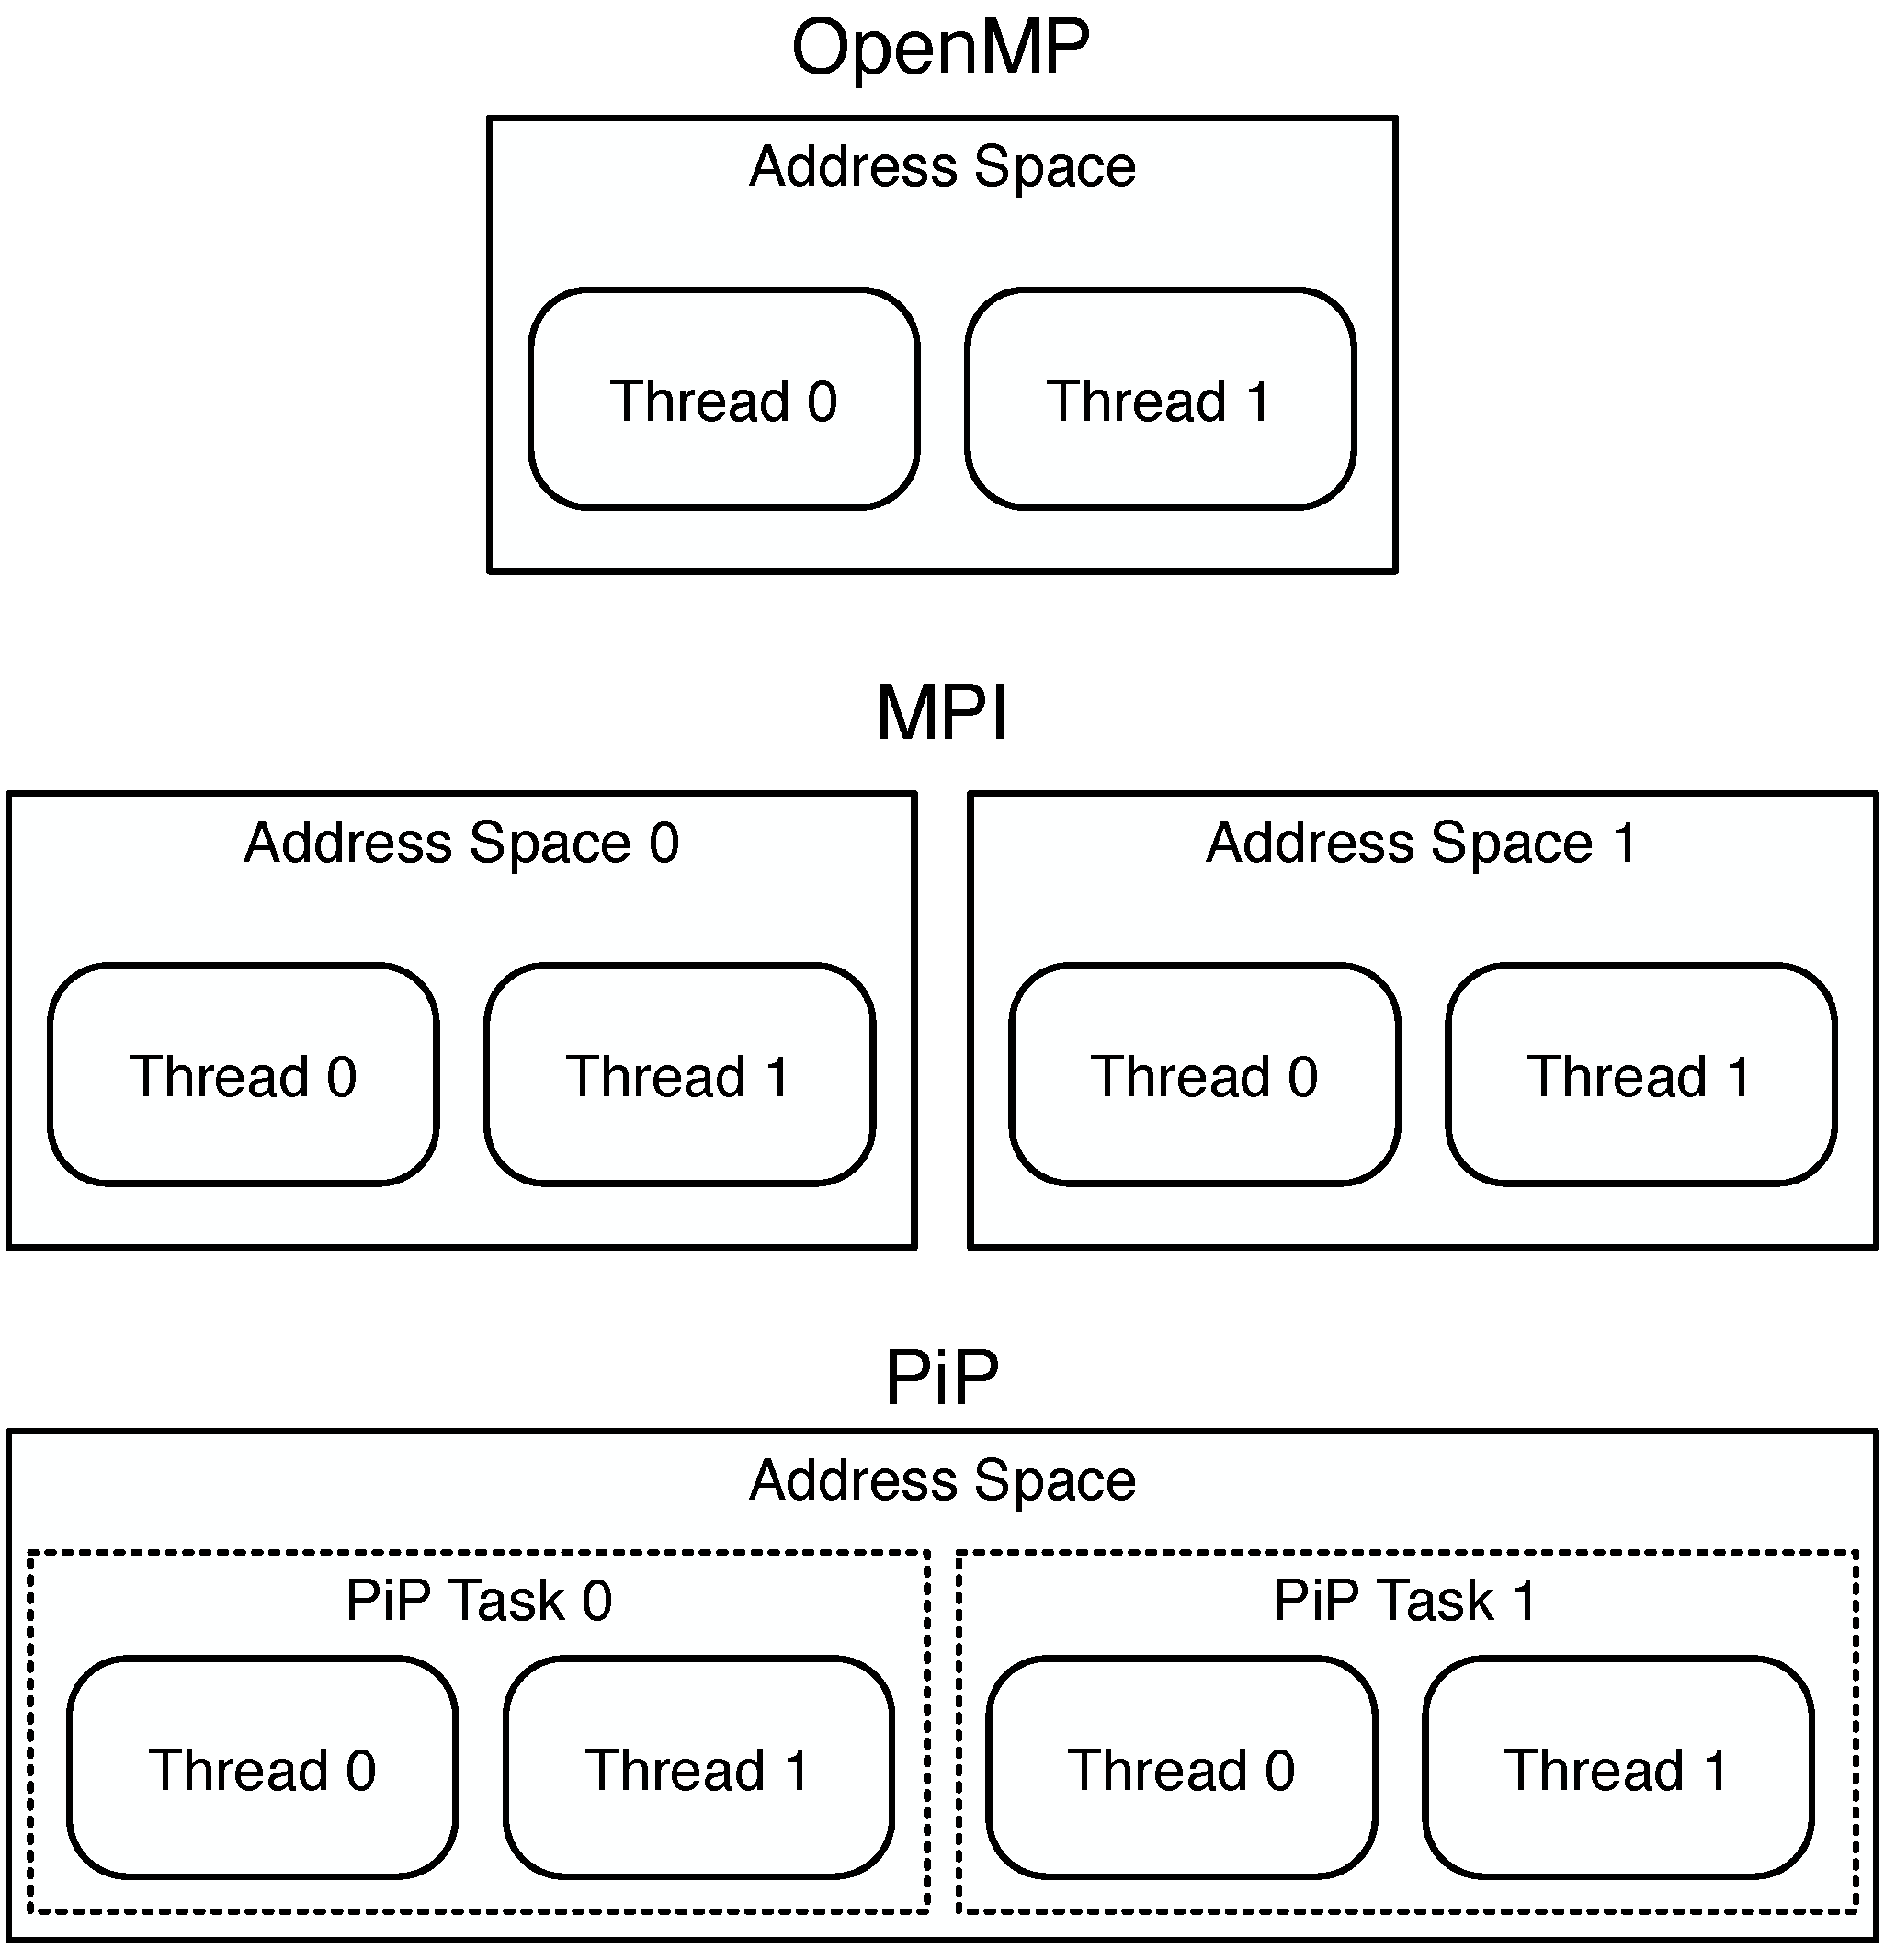
\includegraphics[width=0.7\columnwidth]{tasks/Figs/AddressSpace-OpenMP-MPI-PiP.pdf}
\caption{Differences of OpenMP, MPI and PiP}
\label{fig:tasks:hello-var-omp}
\end{figure}

Static variables are associated to an address space in the traditional
process model and thread model. Because of this, each process has its
own static variables, which are shared by all threads using the same
address space. Each PiP task is guaranteed to have its own static
variable set under the PiP execution model, decoupling from the
address space while maintaining address space sharing. {\it variable
  privatization} is what this is.

It is simple to share information among PiP tasks while maintaining
the independence of each PiP task's execution thanks to the nature of
PiP, which includes privatized variables and sharing an address
space. The ``Hello World'' program has so far been proved to be able to
execute as PiP tasks concurrently, although this program is quite
basic and there is no information exchange between PiP tasks. We'll
demonstrate how information can be shared between PiP processes in the
section after this one.

\subsection{Export and Import}

If the address of the information to be exchanged is known, sharing an
address space allows data owned by a PiP task to be accessed. The
address of the shared data can be broadcast by a PiP task, and the
other PiP task(s) can obtain the published address.  

To start, each PiP task has a {\PIPID} that helps it stand out from the
rest. By giving the {\PIPID} of the exporting PiP task, other PiP tasks
that share the same address space can import the exported address.

\lstinputlisting[style=program,
  caption={Export and Import ({\tt export-import})},
  label=prg:export-import] {tasks/examples/export-import.c}

In this program, after adjusting the value of {\tt argv[1]}, a PiP
task with a PIPID of zero (zero) exports the address of the variable
{\tt x} by using \pipfunc{pip_named_export}. By using the
\pipfunc{pip_named_import} function, the 
remaining PiP tasks import the address that PiP task 0 exported. An
outcome of this program's execution is shown below. The other PiP
tasks can view the value that PiP task 0 exported, as demonstrated.

\lstinputlisting[style=example, 
  caption={Execution of Export and Import},
  label=out:export-import] {tasks/examples/export-import.out}

The address with the specified name is published by the
\pipfunc{pip_named_export} function. The
\pipfunc{pip_named_import} function blocking-waits for the specified
PiP job by {\PIPID} to reach the defined address. To avoid a race condition,
it is not permitted to export an address with the same name more than
once for the purpose of updating the address.

The PiP library's functions almost always return an integer value as
an error code. A return code of zero (zero) denotes success. This
error code is identical to those that Linux defines. Due to simplicity
and clarity, the returned code is not tested in the examples presented
thus far and moving forward.  

It is forbidden in \term{MPI} to access the data that is held by other
processes running on the same node\footnote{Strictly speaking, some
  \term{MPI} implementations based on the thread model may allow
  this. Major \term{MPI} implementation, such MPICH, 
Open MPI, and many other \term{MPI} implementations provided by vendors are
based on the process model, and there is no way to access data owned by
the other \term{MPI process}.}. In MPI, communication is the sole 
permitted method. Communication fundamentally entails copying data in
some way (done by software or hardware). Data copying consumes memory,
power, and time.



\section{Spawning PiP Tasks and Waiting Terminations}

The \pipcomm{pip-exec} command spawns PiP tasks. The
process which spawns PiP tasks is called {\bf (PiP) root} process. The
\pipcomm{pip-exec} process is a PiP root process. 
PiP tasks spawned by the root process are mapped and executed in the
address space of the root. In this chapter, how to spawn PiP tasks
will be explained.

\subsection{Spawning PiP tasks}

\subsubsection{Spawning a program as PiP tasks}

Listing~\ref{prg:spawn-root} is an example of a PiP root program. It
spawns $N$ PiP tasks, where $N$ is specified by the first parameter
of the program. The \pipfunc{pip_init()} function must be called to
initialize the PiP library before calling any other PiP functions,
although there some exceptions to this. The \pipfunc{pip_init()} may
look strange because this function behaves differently depending
on if it is called from a PiP root or PiP task. The first argument is
output returning {\PIPID} of the calling task. The second input
arguments is to specify the maximum number of spawning PiP tasks. This
second argument becomes output if this is called by a PiP task,
returning the number specified by the root.
The \pipfunc{pip_fin()} function works as the opposite of
\pipfunc{pip_init()}, finalizing PiP library and freeing allocated 
resources. After calling \pipfunc{pip_fin()}, most PiP library
functions return an error code (\linuxdef{EPERM}).
\comment{The other arguments will be explained in the
  Section~\ref{sec:advanced}.} 

The \pipfunc{pip_spawn()} function is called after then. The first and
second arguments are the same with the Linux's \linuxfunc{execve()}
function; the first is to specify the executable file to be executed
and the second argument is to specify the parameters executing the
program. The third is to specify environment variables. When it is
{\NULL}, then value of the Glibc global variable \linuxvar{environ} is
taken. Th fourth argument is to specify the CPU core number to bind
the spawned PiP task and which CPU core. In this example, the value of
\pipdef{PIP_CPUCORE_ASIS} means that the (CPU) core-bind should be
the same with the one when calling \pipfunc{pip_spawn()}. The fifth
is an input and output argument and you can specify \PIPID\ or
set to \pipdef{PIP_PIPID_ANY} so that PiP library can choose
any. After calling \pipfunc{pip_spawn()}, the argument returns the
actual \PIPID. 

\lstinputlisting[style=program, caption={Spawn ({\tt spawn-root})},
  label=prg:spawn-root] {spawn/examples/spawn-root.c}

Listing~\ref{prg:spawn-task} is very similar to the ``Hello World''
program in the previous section. The major difference here is calling
the \pipfunc{pip_init()} function. Unlike root, this function call is
optional in the PiP task program. By calling this, you can get 
{\PIPID} and the number of maximum PiP tasks which are specified by the
root. Linsting~\ref{out:spawn} shows an example of the execution of
Listing~\ref{prg:spawn-root} and \ref{prg:spawn-task}. 

\lstinputlisting[style=program, caption={Spawn ({\tt spawn-task})},
  label=prg:spawn-task]
                {spawn/examples/spawn-task.c}

\lstinputlisting[style=example, 
  caption={Spawn - Execution}, label=out:spawn]
                {spawn/examples/spawn.out}

\subsubsection{Spawning myself}

A program can be both or either PiP root and PiP
task. Listing~\ref{prg:spawn-myself} shows an example of combining the
programs of Listing~\ref{prg:spawn-root} and \ref{prg:spawn-task}. We
hope you can understand the strange behavior of \pipfunc{pip_init()}
function. The PiP root process also acts like a PiP task. It has a
special PIPID, \pipdef{PIP_PIPID_ROOT}. 
Listing~\ref{out:spawn-myself} shows the example of this
execution. 

\lstinputlisting[style=program, caption={Spawn Myself ({\tt spawn-myself})},
  label=prg:spawn-myself]
                {spawn/examples/spawn-myself.c}

\lstinputlisting[style=example, 
  caption={Spawn Myself - Execution}, label=out:spawn-myself]
                {spawn/examples/spawn-myself.out}

\subsubsection{Starting from other than {\tt main}}\label{sec:spawn-func}

PiP tasks start from the {\tt main()} function in the examples so
far. PiP allows for PiP tasks to start user-defined function other
than {\tt main()}. In this case, use the \pipfunc{pip_task_spawn()}
function instead of calling the \pipfunc{pip_spawn()} function.

\lstinputlisting[style=program, caption={Starting from user-defined
    function ({\tt userfunc})},
  label=prg:userfunc] {spawn/examples/userfunc.c}

Listing~\ref{prg:userfunc} is the program of this example. To decrease
the number of arguments to spawn a PiP task, the
\pipstruct{pip_spawn_program_t} structure is defined. This structure
holds all information for spawning a program, including path to
executable file, function name, and so on. To hide the details of the
structure, \pipfunc{pip_spawn_from_func()} function is also defined
to set these information. The user-defined function must have one
argument ({\tt void*}) and return an integer value which is the same
as the return value from the {\tt main()} function.

\lstinputlisting[style=example, 
  caption={Starting from user-defined function - Execution},
  label=out:userfunc] {spawn/examples/userfunc.out}

The \pipfunc{pip_spawn()} was firstly introduced (from version
1). After then, I noticed users can start PiP tasks other than main,
and the \pipfunc{pip_task_spawn()} function was
introduced (from version 2 or later). The
\pipstruct{pip_spawn_program_t} structure must be set 
by calling the \pipfunc{pip_spawn_from_main()} function when
starting from the {\tt main()} function. Listing~\ref{prg:mainfunc} is
the program rewritten version of Listing~\ref{prg:spawn-myself} by
using the \pipfunc{pip_task_spawn()} and
\pipfunc{pip_spawn_from_main()}.

\lstinputlisting[style=program, caption={Starting from main
    function ({\tt mainfunc})},
  label=prg:mainfunc]
                {spawn/examples/mainfunc.c}

\lstinputlisting[style=example, 
  caption={Starting from main function - Execution},
  label=out:mainfunc] {spawn/examples/mainfunc.out}


\subsection{Waiting for Terminations of PiP tasks}

As readers may have already noticed, the \pipfunc{pip_wait()} is the
function to wait for terminations of the spawned PiP tasks. The
\pipfunc{pip_wait()} function acts like the Linux's \linuxfunc{wait()}
function. In many cases, Linux's \linuxfunc{wait()} function works
with PiP tasks, but there is a certain case it does not. So, it is
recommended for users to use \pipfunc{pip_wait()} function.

The argument of the \pipfunc{pip_wait()} is the pointer to an integer
variable, the same with the Linux's \linuxfunc{wait()} call. The
returned integer can be examined by using the Linux's
\linuxdef{WIFEXITED}, \linuxdef{WIFSIGNALED}, \linuxdef{WEXITSTATUS},
\linuxdef{WIFSIGNALED}, and \linuxdef{WTERMISIG} macros. 

\lstinputlisting[style=program, caption={Waiting for specified PiP task
    terminations ({\tt wait})}, label=prg:wait]
                {spawn/examples/wait.c}

\lstinputlisting[style=example, 
  caption={Waiting for specified PiP task terminations - Execution},
  label=out:wait] {spawn/examples/wait.out}

\pipfunc{pip_wait()} waits for the PiP task termination specified by
        {\PIPID}. 
\pipfunc{pip_wait_any()} function can wait for any PiP tasks and
        {\PIPID} and exit status are returned when terminated (See
        Listing~\ref{prg:waitany} and \ref{out:waitany}).
        \pipfunc{pip_trywait()} and \pipfunc{pip_trywait_any()} are
        the non-blocking versions of \pipfunc{pip_wait()} and
        \pipfunc{pip_wait_any()}, respectively. 

\lstinputlisting[style=program, caption={Waiting for any PiP task
    terminations ({\tt waitany})}, label=prg:waitany]
                {spawn/examples/waitany.c}

\lstinputlisting[style=example, 
  caption={Waiting for any PiP task terminations - Execution},
  label=out:waitany] {spawn/examples/waitany.out}


\subsection{Terminating PiP tasks}

PiP tasks and root can terminate their executions by calling
\pipfunc{pip_exit()} function. This function acts like the Linux's
        \linuxfunc{exit()} function. As described above, it is recommended
        to use \pipfunc{pip_exit()} 
        instead of \linuxfunc{exit()}, because the Linux's \linuxfunc{exit()}
        function works in most cases, however, there is a case it does
        not. Listing~\ref{prg:exit} and \ref{out:exit} show the
        example showing how \pipfunc{pip_exit()} works.

\lstinputlisting[style=program, caption={PiP Task Termination
    function ({\tt exit})}, label=prg:exit] {spawn/examples/exit.c}

\lstinputlisting[style=example, 
  caption={PiP Task Termination - Execution},
  label=out:exit] {spawn/examples/exit.out}


\section{Timing Synchronization among PiP Tasks}

This section will explain about the timing synchronization among PiP
tasks.

\subsection{Barrier Synchronization}

Currently, there is only one synchronization method is supported by
the PiP library, it is barrier synchronization. The API of PiP's
barrier synchronization is borrowed from the one found in the PThread
library. There are three functions in PiP,
\pipterm{pip_barrier_init()}, \pipterm{pip_barrier_wait()}, and
  \pipterm{pip_barrier_fin()}, corresponding to {\tt
    pthread_barreir_init()}, {\tt pthread_barrier_wait()} and {\tt
        pthread_barrier_destroy()}, respectively. 

\lstinputlisting[style=program, caption={Barrier Synchronization
    ({\tt barrier})}, label=prg:barrier] {sync/examples/barrier.c}

In Listing~\ref{prg:barrier}, the \pipterm{pip_init()} function is
given a new non-{\tt NULL} value to the third argument. This is
another form of exporting a pointer from the root to spawnd PiP
tasks. In this example, the address of the \pipterm{pip_barrier_t}
static variable is passed to children so that the children can
synchronize by calling \pipterm{pip_barrier_wait()}.

To clarify the effect of the barrier synchronization, the
synchronization takes place only when the second parameter of the
program execution is not given, and then the return values of
\pipterm{pip_gettime()} are shown by PiP tasks. The
\pipterm{pip_gettime()} returns the current value of {\tt
  gettimeofday()} in double format with the unit of seconds.

The example of running of this program is shown in
Listing~\ref{out:barrier}. In the first run, the barrier
synchronization does not take place and large variance can be seen on
the {\tt gettimeofday()} values. In the second run, where the barrier
synchronization takes place, and smaller variance can be seen.

\lstinputlisting[style=example,
  caption={Barrier Synchronization - Execution},
  label=out:barrier] {sync/examples/barrier.out}

\subsection{Using PThread Synchronization}

Users can utilize the synchronization functions on PiP tasks provided
by the PThread library. This is simply because PiP tasks share the
same address space, just like threads.

\subsection{\tt pthread_barrier}

The same barrier synchronization can also be implemented by using the
{\tt pthread_barrier} functions. 
Listing~\ref{prg:pthread-barrier} is the program simply replacing
{\tt pip_barrier} functions with the {\tt pthread_barrier} functions.

\lstinputlisting[style=program,
  caption={Pthread Barrier ({\tt
      pthread-barrier})},label=prg:pthread-barrier]
                {sync/examples/pthread-barrier.c}

\lstinputlisting[style=example, 
  caption={Pthread Barrier - Execution}, label=out:pthread-barrier]
                {sync/examples/pthread-barrier.out}
                
\subsection{\tt pthread_mutex}

Similarly, {\tt pthread_mutex} also works with PiP. 

\lstinputlisting[style=program,
  caption={Pthread Mutex ({\tt
      pthread-mutex})},label=prg:pthread-mutex]
                {sync/examples/pthread-mutex.c}

\lstinputlisting[style=example, 
  caption={Pthread Mutex - Execution}, label=out:pthread-mutex]
                {sync/examples/pthread-mutex.out}


\section{\pipterm{pipcc} and \pipterm{pipfc}}

\section{\pipterm{pip-exec}}

\section{\pipterm{pip-check}}

\section{\pipterm{pips}}

\section{\pipterm{pip-mode} and \pipterm{printpipmode}}



\section{Summary}

\subsection*{PiP root and PiP task}

\begin{itemize}
\item PiP programs must be compiled with the \pipcmd{pipcc} 
  (for C and C++) or \pipcmd{pipfc} (for Fortran) command.
\item PiP programs can run as PiP tasks by using the
  \pipcmd{pip-exec} command. 
\item PiP programs can run as non-PiP tasks by invoking them as normal
  programs.
\item Unlike the conventional multi-thread model (i.e. OpenMP), static
  variables in a PiP program are privatized and each PiP task has its
  own set of the static variables.
\item Unlike the conventional multi-process model (i.e. MPI), PiP
  tasks may share the same address space and PiP tasks can access data
  owned by the other PiP tasks. 
\end{itemize}

\subsection*{PiP API}

\begin{itemize}
\item Most PiP functions return error code defined in Linux.
\item Every PiP task has a unique {\PIPID} per address space.
\item PiP root must initialize PiP library by calling
  \pipfunc{pip_init()}. While child PiP task may or may not call the
  initialization function.
\item PiP root can spawn PiP tasks by calling the
  \pipfunc{pip\_spawn()} or \pipfunc{pip_task_spawn()} function.
\item To obtain the address for accessing data of the other PiP tasks,
  use the \pipfunc{pip_named_export()} and
  \pipfunc{pip_named_import()} functions.  
\item The \pipfunc{pip_named_export()} and \pipfunc{pip_named_import()}
  can be used to synchronize tasks. \pipterm{pip_barrier_wait()} can
  also be used for tasks to synchronize.
\item The \pipfunc{pip_exit()} function terminates the calling PiP
  task and PiP root.
\item PiP root can wait for the termination of a spawned PiP task, by
  calling one of the \pipfunc{pip_wait()} function family.
\end{itemize}
 


\section{Some Myths on PiP}

\subsubsection*{Sharing an address with multiple programs can be a
  severe security issue}\label{sec:security-issue}

PiP allows to run programs sharing the same address space. The
most important point here is to make information exchange among
programs easy and efficient. If there is no information exchange among
them, there is no reason to run them with the PiP environment.

Basically, communicating programs share the same fate. Even a most
simple case where two programs are connected by using the Linux/Unix
pipe, one of the programs dies, the other programs also dies by
receiving the {\tt SIGPIPE} signal. Communicating programs agree with
others when to communicate and how to communicate. The PiP case is no
exception.

\subsubsection*{Sharing address space makes debugging difficult}

It is true if one of the processes in a PiP environment destroy the
data owned by the other(s) may lead to a catastrophic result. If this
is done maliciously, then this cannot be avoided (see also
above). If the destruction is triggered by a
software bug, then this might be harder-to-debug than that of
multi-process model.  There are two points here; 1) the higher 
possibility of destructing of actual data, not accessing invalid memory
region ({\tt SIGSEGV}), and 2) there are multiple execution entities.

The ASLR can be some help for the former point. If ASLR is enabled,
then the phenomenons of the bug can vary time to time. The situation
of the latter point is almost the same with the multi-thread case.

Anyway, I have no experiences for having bugs based on this situation
up until now. 

\subsubsection*{My program does not have any static variables and I do
  not need PiP.}

You may write programs without having any static variables. However,
the functions implemented in Glibc have many static variables. Your
runtime system may use some of the Glibc functions. So, in general, it
is very hard to write programs not having any static variables.

\subsubsection*{There must be some hidden overhead for running PiP
  programs}

So far, it is know that there is one overhead which is larger than
the multi-process model. It is address space modification system
calls, such as {\tt mmap()} and {\tt brk()}. This is because any
modification of an address space must be locked inside of the OS
kernel and this lock contention results in larger overhead. This
situation is the same with the multi-thread model and the overhead of
{\tt mmap()} is larger than the multi-process model but almost the
same with the multi-thread model. There is no other known additional
overhead in PiP so far. 


\chapter{PiP Advanced}\label{chap:advanced}

blablabla


\section{Rationale}\label{sec:rationale}

The prosedure to spawn a PiP task is (more detailed procedure can be
found at Section~\ref{sec:spawn-details});

\begin{enumerate}
\item create a new name space by calling the Linux's {\tt dlmopen()}
  function,
\item create a PiP task process (or thread) by calling the Linux's
  {\tt clone()} system call, and 
\item jump into the starting function of a user program.
\end{enumerate}

The {\tt dlmopen()} function can create a new name space, unlike {\tt
  dlopen()}. Here, the {\it name space} is the global symbol names
(functions and global variables) to be resolved at loading a program. By
creating a new name space, functions and variables can be
privatized from the other PiP tasks. 

The order of calling the {\tt dlmopen()} and {\tt clone()} is very
important.  At first, I tried to call them in the order of calling
{\tt clone()} followed by {\tt dlmopen()}, because this way seemed to be
quite natural, however, this does not work at all. This the reason of
that only PiP root can spawn PiP tasks and wait for the terminations
of PiP tasks. 

In some cases (or, in most cases before CentOS/Redhat 8), the loaded
address of a program is fixed by default. If this is the case, PiP
cannot load multiple programs in the same address space. To enable
this, the PiP executables must be compiled as \PIE\ (Position
Independent Executable) so that the programs can be loaded at any
arbitrary address. All programs to be PiP tasks must be compiled as
\PIE, i.e., must be compiled with \pipterm{pipcc} or \pipterm{pipfc}
with the {\tt --piptask} option (or nothing to use the default). Note
that PiP root program may not be \PIE.  

By running the loaded program having a new name space with another
thread, PiP task can be created. Unfortunately, things are not that
simple. There are many issues coming from Glibc. The next section will
describe these issues. 


\section{Issues related to Linux Kernel and Glibc}

This section will explain about the issues when implementing PiP. 

\subsection{Loading a Program}

Before going into the details about the Glibc issues when implementing
PiP, readers should understand how a program is loaded into
memory. This subsection describes only about the program loading
procedure of Linux, apart from PiP implementation.

When the Linux's {\tt execve()} system call to run a program, the
Linux kernel open and read the executable file, searching the ELF
section named ``{\tt .interp}.''

\lstinputlisting[style=example, basicstyle=\tiny\tt, 
  caption={{\tt .interp} Section of the {\tt ps} command},
  label=out:interp] {glibc/examples/interp.out}

Listing~\ref{out:interp} shows the value of the {\tt .interp} section,
{\tt /lib64/ld-linux-x86-64.so.2}. The Linux kernel
invokes the loader specified by the {\tt .interp} section and asks the
loader to load a program specified by the {\tt execve()} parameter.
Then the loader load the program and additionally load and link the shared
libraries required to run the program. Once everything is loaded, the
loader jumps into the starting function defined in Glibc to initialize
Glibc and finally user-defined {\tt main()} function is called.

The program loader, often simply called {\tt ld-linux.so}, is loaded
once per address space and kept in memory until the end of the
process. This is responsible for any loading process by resolving the
external symbol references. The Glibc functions defined in the {\tt
  libdl.so} ({\tt -ldl}), such as {\tt   dlopen()}, {\tt
  dlmopen()}, {\tt dlsym()} and so on, are just API 
and their functional bodies exist in the program loader.

\subsection{PiP-glibc}

PiP provides a new execution model which cannot be categorized into
neither the process model nor the thread model. In this new model,
although its name is not yet given, tasks share the same address
space like the thread model, but maintaining the variable
privatization like the process model. This execution
model is novel and not yet recognized by most of the tool chains
provided by Linux and others. Indeed, the most of the time to develop
PiP was devoted to find niches in Glibc.

\subsubsection{Number of name spaces}

The number of names spaces which the {\tt dlmopen()} can create is
hard-coded as 16. Considering PiP tasks run in parallel and the number
of CPU cores nowadays, this number of 16 is apparently too small. The
PiP package provides PiP-glibc where the number of name spaces is
increased, up to 300 PiP tasks\footnote{Once I asked Glibc
development members to increae the size, but they did not accept. Refer
\url{https://sourceware.org/bugzilla/show_bug.cgi?id=23978}}. 

The name space table resides in the {\tt ld-linux.so} and this means
that the {\tt .interp} ELF section of PiP programs must be changed so
that the program is loaded by the new {\tt ld-linux.so}. This can be
done by specifying {\tt --dynamic-linker} option of the GNU linker and
the \pipterm{pipcc} and \pipterm{pipfc} do this.

The name space table resides at the top of a structure in {\tt
  ld-linux.so}. Some Glibc functions refer to the members in this
structure directly. This causes another problem. Once the size of the
name space table is changed, the addresses of the other members in the
same structure are also changes. As described, only one {\tt
  ld-linux.so} can be loaded in an address space. As a result, all PiP 
programs sharing the same address must be linked with the same Glibc. 

\subsubsection{PiP-gdb}

The {\tt ld-linux.so} embeds a tiny information for debugging into the
loaded program. Unfortunately, I found that this code fragment
resides on the pass calling the {\tt ld-linux.so} from the
top (by the kernel), not on the pass called from {\tt dlopen()}
  and {\tt dlmopen()}\footnote{I guess the loaded code by using {\tt
    dlopen()} or {\tt dlmopen()} cannot be debugged.}. The patched
  PiP-glibc fixed this issue. Thus, the \pipterm{pip-gdb} command
  (Section~\ref{sec:pip-gdb}) can only work with 
  the PiP programs linked with the patched PiP-gkibc.

\subsubsection{Global lock}

Most programs are linked with Glibc and PiP programs are no
exception. PiP allows to run multiple PiP programs in the same address
space. This means that each PiP task has its own Glibc. And the
simultaneous calls of some Glibc functions may not work because of a
race condition. 

To avoid this condition, PiP library provides the functions,
\pipterm{pip_glibc_lock()} and \pipterm{pip_glibc_unlock()}, to 
serialize the Gilbc function calls. The following Glibc functions are
wrapped by PiP library to introduce the lock and users do not have to
care the race. 

\begin{table}[ht]
  \centering
  \caption{Glibc functions wrapped by PiP library}
  \vspace{3mm}
  \tt
  \begin{tabular}{lll}
    \hline
    dlsym	&
    dlopen	&
    dlmopen	\\
    dlinfo	&
    dlclose	&
    dlerror	\\
    dladdr	&
    dlvsym	&
    getaddrinfo	\\
    freeaddrinfo &
    gai_strerror &
    pthread_create \\
    \hline
    pthread_exit \\
    \hline
    malloc 	&
    free	&
    calloc	\\
    realloc	&
    memalign 	&
    posix_memalign \\
    \hline
  \end{tabular}
\end{table}

The functions {\tt pthread\_exit()} and below of this have another
reason to have function wrapper. The wrapping reason of {\tt
  pthread\_exit()} will be explained in the
Section~\ref{sec:exec-mode} and the reason of wrapping malloc routines
will be explained in Section~\ref{sec:malloc}. 

These listed functions may not be complete. There can
be a case where some other Glibc functions may suffer from the
race condition. This problem can be avoided by introducing the above
locking functions. This lock can be used recursively and users can
avoid deadlock situation easily. 

\subsubsection{\PIPKW{pip-unpie} program}

The Glibc in CentOS/RedHat 8 (and possibly newer ones) does not allow
to load a program by the {\tt dlmopen()} function\footnote{Refer
\url{https://sourceware.org/bugzilla/show_bug.cgi?id=11754\#c15}}. The
\pipterm{pip-unpie} program is to cheat this Glibc restriction. This
program is automatically executed by the \pipterm{pipcc} or
\pipterm{pipfc} when creating a PiP executable, and not to be invoked
by users directly.

\subsubsection{Constructors and Destructors}

The constructors and destructors are used in C++
programs. Constructors and destructors are list of
functions. Generally, constructor functions are called just before the 
program begins, and destructors functions are called when the program
is about to exit.

In PiP, the behavior of the constructors and destructors is
somewhat different. To explain this, I should start explaining how the
constructors and destructors are implemented in general. The
constructor functions are listed in the {\tt .init_array} section of an ELF
file. The destructor functions are listed in the {\tt .fini_array}
section. Constructors are called when {\tt ld-linux.so} finishes
loading and linking objects. Destructors are called when {\tt
  dlclose()} is called.

Now back to PiP. As described in 

\subsection{Linux Kernel}

%\subsubsection{Heap Segment and Address Space}

There is another issue which comes from Linux kernel, not from
Glibc. Before explaining this issue, let us start from the how an
address space is composed. 

\lstinputlisting[style=example, basicstyle=\tiny\tt, 
  caption={A Memory Map Example},
  label=out:maps] {glibc/examples/maps.out}

Listing~\ref{out:maps} shows an example of the output of doing ``{\tt
  cat /proc/$\langle$PID$\rangle$/maps}.'' Here, ``{\tt pip-exec -n 2
  ./a.out}'' was executed, resulting one \pipterm{pip-exec} process
and two {\tt ./a.out} tasks. The file, {\tt
  /proc/$\langle$PID$\rangle$/maps}, lists all memory
segments in an address space of the process {\tt $\langle$PID$\rangle$}
usually. A loaded shared object has consecutive three or four segments; 
executable, gap (not accessible, if any), constants and data. 
The rightmost column of a line indicates the {\tt
  mmap()}ed filename, the second from the left column indicates the
permission of the memory segment. '{\tt r}' is readable, '{\tt w}' is
writable, '{\tt x}' is executable and '{\tt p}' is private
(copy-on-write). There are also some special segments whose filename
is in a pair of square brackets; {\tt [stack]}, {\tt [heap]}, and so
on. These are created by the Linux kernel for special purposes as
their names suggest. The segments having no filename are created by
the {\tt mmap()} system call. 

Remember, this is the address space of running one PiP root and two PiP
tasks, resulting to have all the segments of the three tasks. Usually,
the heap segment, mainly used for {\tt malloc()}, exists only one per
address space. As shown in this example, there is only one heap
segment, meaning the heap segment is shared by three tasks (one for
root and two for PiP tasks). Note that the all three tasks have
exactly the same {\tt /proc/$\langle$PID$\rangle$/maps} content, and
there are three sets of a shared library and only one set of {\tt
  ld-linux.so} ({\tt ld-2.28.so}) can be seen in
Listing~\ref{out:maps}.  

The heap memory can be allocated or deallocated by calling the {\tt
  brk()} system call. Usually, there are two calls of {\tt brk()} to
allocate or deallocate heap memory, one for obtaining the current heap
end address and another for setting the new heap end
address. Unfortunately, this API is not thread-safe at all, and thus,
the heap memory cannot be used safely by PiP tasks.

Fortunately, the malloc routines in Glibc is designed to check if
there are two or more name spaces and if so they do not use the {\tt
  brk()} system call, use {\tt mmap()} instead. So, the Glibc malloc
routines work with PiP without a problem. However, if some other
routines use the {\tt brk()} system call (or {\tt sbrk()} Glibc
function), for example, replacing the Glibc malloc routines with
another malloc implementation, then this may result in a problem. 


\section{Execution Mode}\label{sec:exec-mode}

PiP library is made to function on Linux. According to
Section~\ref{sec:rationale}, it is very dependent on the
\linuxfunc{dlmopen} and \linuxfunc{clone} functions. Particularly, the
\linuxfunc{clone} function is called with a unique set of 
{\tt CLONE} flags. Many Linux variants exist, and some of them do not
support the specified {\tt CLONE} flag combination (for example,
McKernel\footnote{\url{https://github.com/ihkmckernel/mckernel}}). There
are two ways to execute PiP in such an environment: 
one involves executing \linuxfunc{clone} with a particular flag
combination, and the other involves calling \linuxfunc{pthread_create}
to start a PiP task while 
using the standard {\tt CLONE} flag combination. \pipterm{Process
  mode} refers to the former and \pipterm{pthread mode} to the
latter. Both modes keep the fundamental characteristics of the PiP,
including address space sharing and 
flexible privatization.

\subsection{Differences Between Two Modes}

{\tt CLONE} flag combinations ultimately determine the difference in the
PiP execution mode. The {\tt CLONE} flag values \linuxdef{CLONE_FS},
\linuxdef{CLONE_FILES}, \linuxdef{CLONE_SIGHAND}, and
\linuxdef{CLONE_THREAD} are reset, but \linuxdef{CLONE_VM} and
\linuxdef{CLONE_SYSVSEM} are set, in contrast to the 
pthread mode. 

\begin{table}[ht]
  \centering
  \caption{Differences between two modes}\label{tbl:mode-diff}
  \vspace{3mm}
  \begin{tabular}{c||c|c}
    \hline
    & Process Mode & Pthread Mode \\
    \hline
    \hline
    Address Space Sharing & yes & yes \\
    Variable Privatization & yes & yes \\
    File Descriptors (FDs) & not shared & shared \\
    \hline
  \end{tabular}
\end{table}

The primary distinctions between the two modes are shown in
Table~\ref{tbl:mode-diff}. There are a lot more variations, however
the PiP library offers mode-agnostic functions so that users can
develop PiP programs without worrying about the variations in mode.

\begin{table}[ht]
  \centering
  \caption{Mode-Agnostic Functions}\label{tbl:mode-agnostic}
  \vspace{3mm}
  \small
  \begin{tabular}{c||c|c||l}
    \hline
    Mode-Agnostic & Process Mode & Pthread Mode & \multicolumn{1}{c}{note} \\
    \hline
    \pipfunc{pip_exit()} & {\tt exit()} & {\tt pthread_exit()} &
    termination \\
    \pipfunc{pip_wait()} & {\tt wait()} & {\tt pthread_join()} &
    {\tiny wait termination} \\
    \pipfunc{pip_kill()} & {\tt kill()} & {\tt pthread_kill()} & send
    signal \\
    \pipfunc{pip_sigmask()} & {\tt sigprocmask()} & {\tt
      pthread_sigmask()} & signal mask \\
    \pipfunc{pip_signal_wait()} & sigwait() & sigwait() & wait signal
    \\
    \pipfunc{pip_yield()} & {\tt sched_yield()} & {\tt
      pthread_yield()} & yield \\
%%    \pipterm{pip_abort()} & {\tt abort()} & {\tt abort()} & kill all
%%    tasks \\
    \hline
  \end{tabular}
\end{table}

There are also predicate functions for users to know the current
mode listed in Table~\ref{tbl:mode-predicates}.

\begin{table}[ht]
  \centering
  \caption{Execution Mode Predicates}\label{tbl:mode-predicates}
  \vspace{3mm}
  \begin{tabular}{c|c}
    \hline
    Function name & \multicolumn{1}{c}{note} \\
    \hline
    \pipfunc{pip_is_threaded()} & if pthread mode \\
    \pipfunc{pip_is_shared_fd()} & if FDs are shared \\
    \hline
  \end{tabular}
\end{table}

In the current implementation, \pipfunc{pip_is_threaded} and
\pipfunc{pip_is_shared_fd} have the same meaning. There may be
situations in which those two terms have different meanings, so having
those functions is necessary. 

\subsection{How to Specify Execution Mode}

When calling \pipfunc{pip_init} or setting the \pipenv{PIP_MODE}
environment variable at runtime, the execution mode can be
selected. The function prototype 
for the \pipfunc{pip_init} shown below. Up until this point, the first
three arguments have been discussed.

\begin{lstlisting}[frame=tRBl]
int pip_init( int *pipidp,	[IN/OUT]
              int *ntasksp,     [IN/OUT]
              void **root_expp, [IN/OUT]
              int opts );       [IN]
\end{lstlisting}

The final opts parameter can take one of the following values:
\pipdef{PIP_MODE_PROCESS}, \pipdef{PIP_MODE_THREAD}, or both, or
zero. Zero has the same value as {\tt
  \pipdef{PIP_MODE_PROCESS}|\pipdef{PIP_MODE_PTHREAD}}. The
\pipenv{PIP_MODE} environment can be a string that contains the words
"{\tt process}" or "{\tt pthread}." The value of the \pipenv{PIP_MODE}
environment variable is checked when the opts value is zero or the
value of either oring the two. If no environment is specified, the PiP
library picks a suitable one. The environmental value and the ethical
worth cannot be at odds with one another. 



\section{Spawning Task - Advanced}\label{sec:spawn-adv}

In this section, other features, not described so far, of
\pipterm{pip_spawn()} and \pipterm{pip_task_spawn()} will be
explained. For convenience, the function prototypes of these functions
are shown below;

\begin{lstlisting}[frame=tb]
int pip_task_spawn( pip_spawn_program_t *progp, [IN]
                    uint32_t coreno,            [IN]
		    uint32_t opts,              [IN]
		    int *pipidp,                [IN/OUT]
		    pip_spawn_hook_t *hookp );  [IN]

int pip_spawn( char *filename,                  [IN]
               char **argv,                     [IN]
               char **envv,                     [IN]
	       int coreno,                      [IN]
               int *pipidp,                     [IN/OUT]
	       pip_spawnhook_t before,          [IN]
               pip_spawnhook_t after,           [IN]
               void *hookarg );                 [IN]
\end{lstlisting}

The first argument of \pipterm{pip_task_spawn()} function is already
described in Section~\ref{sec:spawn-func}. This is structure is to
pack the first three arguments of \pipterm{pip_spawn()}. 

\subsection{CPU Core Binding}

The {\tt coreno} argument is to bind the spawned PiP task to the
specified CPU core. By default, this is the $N$th core number. If
users want to specify the absolute core number, then the absolute core
number should be {\tt OR}ed with
\pipterm{PIP_CPUCORE_ABS}\footnote{This is because the core numbers
are not contiguous on some CPU architecture, i.e., Fujitsu A64FX CPU.}
Or, it can be \pipterm{PIP_CPUCORE_ASIS} not to bind.

\subsection{Execution Context}

Before explaining the rest of the arguments, readers should know about
the execution context under PiP. The execution context can be defined
as the state of CPU, i.e., contents of hardware registers. On PiP,
this definition may not be enough. Let us have an example. Suppose
that the same program runs as two PiP tasks and this program has a
function {\tt foo()}. By passing the function pointer, by using the
\pipterm{pip_named_export()} and \pipterm{pip_named_import()}, one of
the PiP task can call the function of the other PiP
task. Additionally, this function accesses a static variable, say {\tt
  var}. If task $A$ calls function {\tt foo} of task $B$, then the
called function accesses the variable owned by task $B$, not $A$.

Thus, the execution context in PiP environment is different from the
one in common sense and some times can become very subtle. In the PiP
library, this happens quite often and makes debugging difficult.

Further, the situation described above, i.e., the association of
static variables and function address, deeply depends on the CPU
architecture and tool chain. The above description is true on  {\tt
  X86_64} and {\tt AArch64}, however, not true on {\tt X86_32}. Thus,
it is not recommended do this.

\subsection{Constructors and Destructors}

\lstinputlisting[style=program,
  caption={Constructors and Destructors},
  label=prg:const-dest] {spawn-adv/examples/const-dest.c}

\lstinputlisting[style=example, 
  caption={Constructors and Destructors - Execution}, label=out:const-dest]
                {spawn-adv/examples/const-dest.out}


\subsection{Hooks}

The last argument of \pipterm{pip_task_spawn()} is the structure
packing the last three arguments of \pipterm{pip_spawn()}. The
\pipterm{pip_spawn_hook_t} structure can be set by calling
\pipterm{pip_spawn_hook()} function. Here is the prototype;

\begin{lstlisting}[frame=tb]
void pip_spawn_hook( pip_spawn_hook_t *hook,  [OUT]
		     pip_spawnhook_t before,  [IN]
		     pip_spawnhook_t after,   [IN]
		     void *hookarg ) {        [IN]
typedef int (*pip_spawnhook_t)( void* );
\end{lstlisting}

The {\tt before}function specified by this structure is called when a
PiP task is created and just before calling the start function (i.e.,
{\tt main()}). And the {\tt after} function is called when the PiP
task is about to terminate. Both functions are called with the argument
specified by the {\tt hookarg} to pass any arbitrary data. 

Usually, new process is created by calling {\tt fork()} and {\tt
execve()} in Linux/Unix. Here, file descriptors owned by
parent process are passed to the created child. In many cases, those
file descriptors are closed or duplicated (see also the next
subsection) and some other settings are done between the calls of {\tt
  fork()} and {\tt execve()}. In PiP, however, the task is created
by one function and there is no chance to do the same setting when
using {\tt fork} and {\tt exec}. 

The execution of those hook functions are done by root with the root
context. As described in Section~\ref{sec:rationale}, {\tt dlmopen()}
is called by the root. Here is an example of this;



\section{File Descriptors}

In the process execution mode, file descriptors of the root process
are passed to the spawned child. In the pthread mode, files
descriptors are simply shared among PiP root and PiP tasks.

If the close-on-exec flag of a file descriptor is set in process mode,
then the file descriptor is closed before calling the before hook
described above or before jump into the start function. 


\subsection{Debugging Support}


\section{Execution Context}\label{sec:context}

Before explaining the rest of the arguments, readers should know about
the execution context under PiP. The execution context can be defined
as the state of CPU, i.e., contents of hardware registers. On PiP,
this definition may not be enough. Let us have an example. Suppose
that the same program runs as two PiP tasks and this program has a
function {\tt foo()}. By passing the function pointer, by using the
\pipfunc{pip_named_export()} and \pipfunc{pip_named_import()}, one of
the PiP task can call the function of the other PiP
task. Additionally, this function accesses a static variable, say {\tt
  var}. If task $A$ calls function {\tt foo} of task $B$, then the
called function accesses the variable owned by task $B$, not $A$
(Listing~\ref{prg:context} and \ref{out:context}).

\lstinputlisting[style=program,
  caption={Function Call of Another Task},
  label=prg:context] {context/examples/context.c}

In this example program, sorry, this goes off the side road,
\pipfunc{pip_named_export()} and 
\pipfunc{pip_named_import()} are called differently than
before. The final argument of these functions is actually a format
string, just like {\tt printf()}, followed by argument(s) needed by
the format. 

\lstinputlisting[style=example, 
  caption={Function Call of Another Task - Execution}, label=out:context]
                {context/examples/context.out}

Thus, the execution context in PiP environment might be different from
the one in common sense and some times its behavior becomes very
subtle. In the PiP library, this happens quite often and makes
debugging difficult. 

Further, the association of static variables and function addresses
heavily depends on the CPU architecture and tool chain. The above
description is true on \AMD and \ARM,
however, not true on \INTEL. Thus, it is not recommended
do this. 

\subsubsection*{Rationale}

Some readers may wonder why this happens. Let me explain this. This
trick is hidden in the address map. Listing~\ref{out:glibc-segs} shows
a part of address map running three tasks, focusing on the Glibc ({\tt
  /lib64/libc-2.28.so}) segments. 

\begin{lstlisting}[basicstyle=\tiny\tt, frame=tRBl, label=out:glibc-segs]
  ...
7ffff53f8000-7ffff55a4000 r-xp 00000000 fe:01 3049686    /lib64/libc-2.28.so
7ffff55a4000-7ffff57a4000 ---p 001ac000 fe:01 3049686    /lib64/libc-2.28.so
7ffff57a4000-7ffff57a8000 r--p 001ac000 fe:01 3049686    /lib64/libc-2.28.so
7ffff57a8000-7ffff57aa000 rw-p 001b0000 fe:01 3049686    /lib64/libc-2.28.so
  ...
7ffff69f6000-7ffff6ba2000 r-xp 00000000 fe:01 3049686    /lib64/libc-2.28.so
7ffff6ba2000-7ffff6da2000 ---p 001ac000 fe:01 3049686    /lib64/libc-2.28.so
7ffff6da2000-7ffff6da6000 r--p 001ac000 fe:01 3049686    /lib64/libc-2.28.so
7ffff6da6000-7ffff6da8000 rw-p 001b0000 fe:01 3049686    /lib64/libc-2.28.so
...
7ffff73d5000-7ffff7581000 r-xp 00000000 fe:01 3049686    /lib64/libc-2.28.so
7ffff7581000-7ffff7781000 ---p 001ac000 fe:01 3049686    /lib64/libc-2.28.so
7ffff7781000-7ffff7785000 r--p 001ac000 fe:01 3049686    /lib64/libc-2.28.so
7ffff7785000-7ffff7787000 rw-p 001b0000 fe:01 3049686    /lib64/libc-2.28.so
  ...
\end{lstlisting}

There are three sets of Glibc segments. The static variables are
located on the last (readable and writable) segment of each set. A
static variable is accessed by an instruction using the offset from
the instruction (program counter relative addressing mode) to the
variable. Thus, the gap size between the code segment (top of the set)
and variable segment (bottom of the set) is important to make all
offsets constant and thus all gap sizes must be the same. In this way,
variables and instructions are associated in \PIE\footnote{This is
not the case if not compiled as \PIE.}, and \PIE\ programs and shared
objects compiled with the \PIC\ option can be loaded at any locations.

Unfortunately, this addressing mode is not supported by all CPU
architectures\footnote{Listing~\ref{out:context} is obtained by
running the program on an \AMD CPU.}. For example, \INTEL 
does not. On this architecture, one general purpose
register is sacrificed to point the variable segment, resulting
performance degradation by loosing one general purpose register. And
the program shown in Listing~\ref{prg:context} exhibits differently. 


\section{Debugging Support}

Some environment variable settings may help debugging PiP programs.

\subsection{\PIPKW{PIP_STOP_ON_START}}

This environment variable is to stop (by sending {\tt SIGSTOP} to
spawned PiP task just before calling the \pipterm{before hook} (if
any). The value of this environment must meet the following format;

\begin{lstlisting}[frame=tb]
  PIP_STOP_START=[<commandfile>]@<PIPID>
\end{lstlisting}

The optional {\tt\option{commandfile}} is a command file or shell
script to be executed on the suspension, and {\tt\option{N}} is the
PIPID to be suspended. If {\tt\option{N}} is -1, then all spawned PiP
tasks will be stopped. The {\tt\option{commandfile}} is invoked with
parameters; PID and PIPID of the PiP task, and a path to the program
of the task.

\lstinputlisting[style=program,
  caption={Stop-on-start Script Example},
  label=prg:stop-on-start] {debug/examples/onstart.cmd}

Listing~\ref{prg:stop-on-start} shows an example of the script for the
\pipterm{PIP_STOP_ON_START}. Here, \pipterm{pips} command is invoked
instead of some debugging command\footnote{All examples are executed
on a Docker environment but {\tt ptrace} (and other commands using
{\tt ptrace}) was unable to run in this example even withthe {\tt
  --cap-add=SYS_PTRACE} Docker option (I confirmed {\tt gdb} worked). So 
\pipterm{pips} was used instead in this example.}. Note that 
the target task is already stopped by the {\tt SIGSTOP}
signal. Somehow you have to explicitly deliver the {\tt SIGCONT}
signal to the task if you want to resume the
task. Listing~\ref{out:stop-on-start} shows the result of 
\pipterm{PIP_STOP_ON_START} execution with this script file. 

\lstinputlisting[style=example, basicstyle=\tiny\tt, 
  caption={Stop-on-start Script Example - Execution},
  label=out:stop-on-start] {debug/examples/stop-on-start.out}

\subsection{\PIPKW{PIP_GDB_SIGNALS}}

This environment variable \pipterm{PIP_GDB_SIGNALS} is to set the
signals to trigger some actions by specifying the
\pipterm{PIP_SHOW_MAPS} and \pipterm{PIP_SHOW_PIPS}, followed by
PiP-gdb invocation. The value of this environment is as follows;

\begin{lstlisting}[frame=tb]
  PIP_GDB_SIGNALS=[ <SIGNAME> ] { "+"|"-" <SIGNAME> }
\end{lstlisting}

The possible {\tt\option{SIGNAME}} vale are listed below;

\begin{table}[ht]
  \centering
  \caption{Possible Signal Names for \pipterm{PIP_GDB_SIGNALS}}
  \vspace{3mm}
  \tt
  \begin{tabular}{l}
    SIGHUP \\
    SIGINT \\
    SIGQUIT \\
    SIGILL \\
    SIGABRT \\
    SIGFPE \\
    SIGINT \\
    SIGSEGV \\
    SIGPIPE \\
    SIGUSR1 \\
    SIGUSR2 \\
    ALL \\
  \end{tabular}
\end{table}

Here, {\tt ``ALL''} means all signals list in this table. Each signal
name in this table can be concatenated by using the plus (+) and/or
minus (-) symbols.  For example, ``{\tt ALL-SIGUSR1}'' indicates the
all signals excluding {\tt SIGUSR1}. ``{\tt SIGUSR1+SIGUSR2+SIGINT}''
represents {\tt SIGUSR1}, {\tt SIGUSR2} and {\tt SIGINT}. 

\subsection{\PIPKW{PIP_SHOW_MAPS}}

If \pipterm{PIP_SHOW_MAPS} environment is set to ``{\tt on}'' and the
a signal specified by the \pipterm{PIP_GDB_SIGNALS} is delivered, then
the address map (Listing~\ref{out:maps}, for example) will be shown. 

\subsection{\PIPKW{PIP_SHOW_PIPS}}

If \pipterm{PIP_SHOW_PIPS} environment is set to ``{\tt on}'' and the
a signal specified by the \pipterm{PIP_GDB_SIGNALS} is delivered, then
\pipterm{pips} command (Section~\ref{sec:pips}) is invoked to show the
status of the other PiP tasks in the same address space.

\subsection{\PIPKW{PIP_GDB_PATH} and \PIPKW{PIP_GDB_COMMAND} (\pipterm{%
process mode} only)}

When \pipterm{PIP_GDB_PATH} is set to the path to \pipterm{pip-gdb}
a signal specified by the \pipterm{PIP_GDB_SIGNALS} is delivered, then
PiP gdb (Section~\ref{sec:pip-gdb}) will be invoked. If the value of
the \pipterm{PIP_GDB_COMMAND} environment is set to a valid filename
and if the filename contains some GDB commands, then PiP-gdb will be
invoked to work with this command file. 


\section{Malloc routines}\label{sec:malloc}

Consider creating a producer-consumer program using PiP, where one PiP
task serves as the producer and another as the consumer. In contrast
to the traditional process approach, PiP does not require an IPC
(Inter Process Communication) system call. Passing pointers pointing
at data to be transmitted from the producer to the consumer is all
that is necessary.  

There is a problem here. If the given data was allocated by the
\linuxfunc{malloc} function, the consumer will \linuxfunc{free} the
passed data. As previously mentioned, each PiP task has a unique set
of \linuxfunc{malloc} and \linuxfunc{free} procedures connected to
static variables that hold and manage a memory pool. When it is no
longer required, the consumer tries to \linuxfunc{free} the data it
has obtained from the producer's memory pool. Unfortunately, 
because the consumer's \linuxfunc{free} procedure is unaware of the
memory space that the producer allocated, it fails
(Figure~\ref{fig:cross-malloc-free-issue}). I gave this circumstance
the moniker {\it cross-malloc-free}. 

\begin{figure}[ht]
\centering
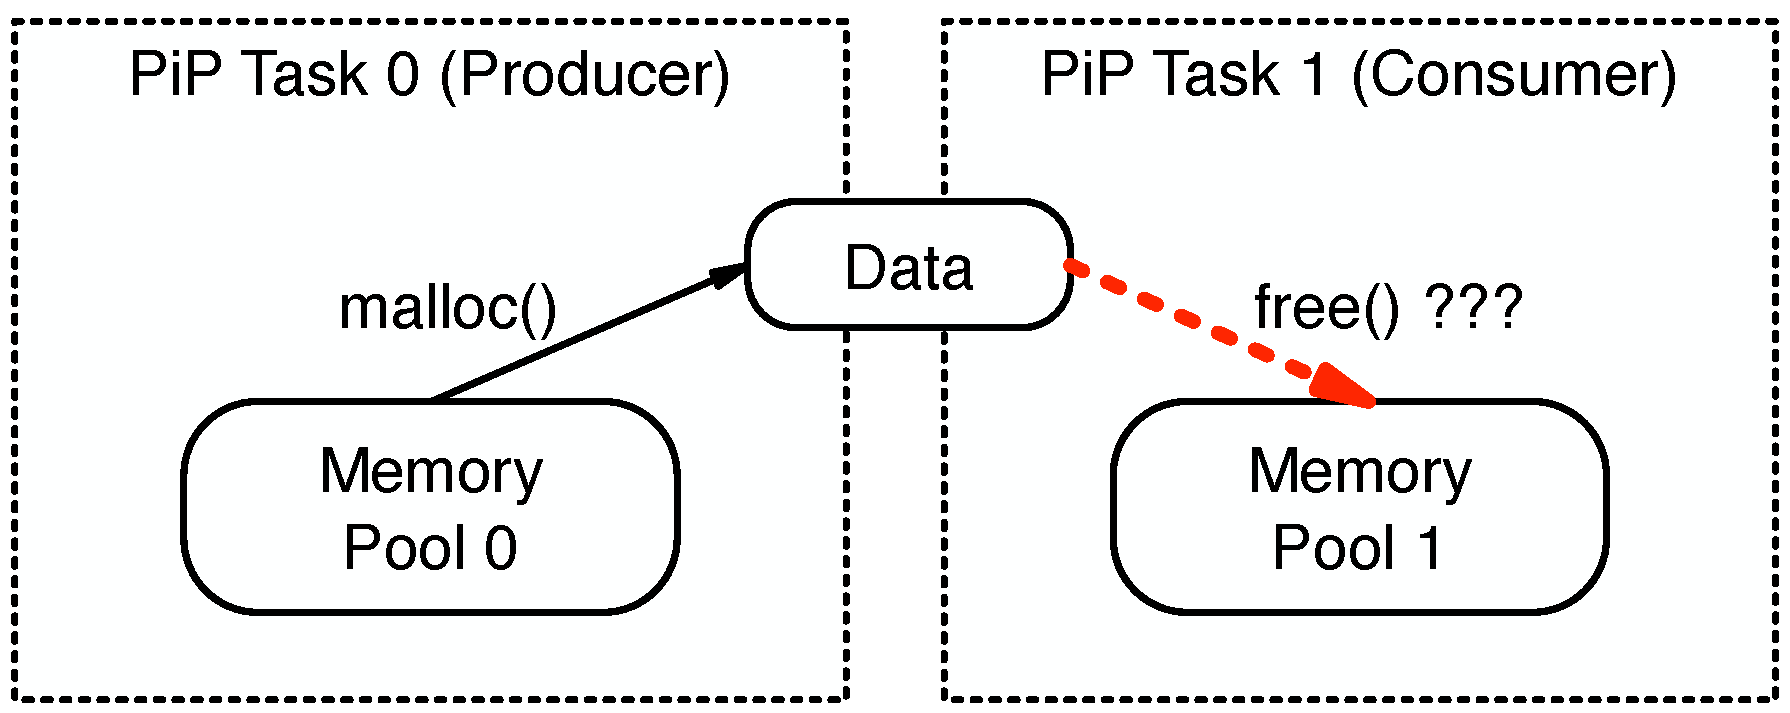
\includegraphics[width=0.7\columnwidth]{malloc/Figs/ProducerConsumer.pdf}
\caption{Cross-Malloc-Free Issue}
\label{fig:cross-malloc-free-issue}
\end{figure}

I gave it a shot using the {\tt malloc} functions that Glibc provides
and discovered that while it doesn't always work, it usually does. I'm
not sure why this works (again, {\it in most circumstances}) with the 
Glibc {\tt malloc} routines, but I believe it's important to avoid
this circumstance.

\begin{figure}[ht]
\centering
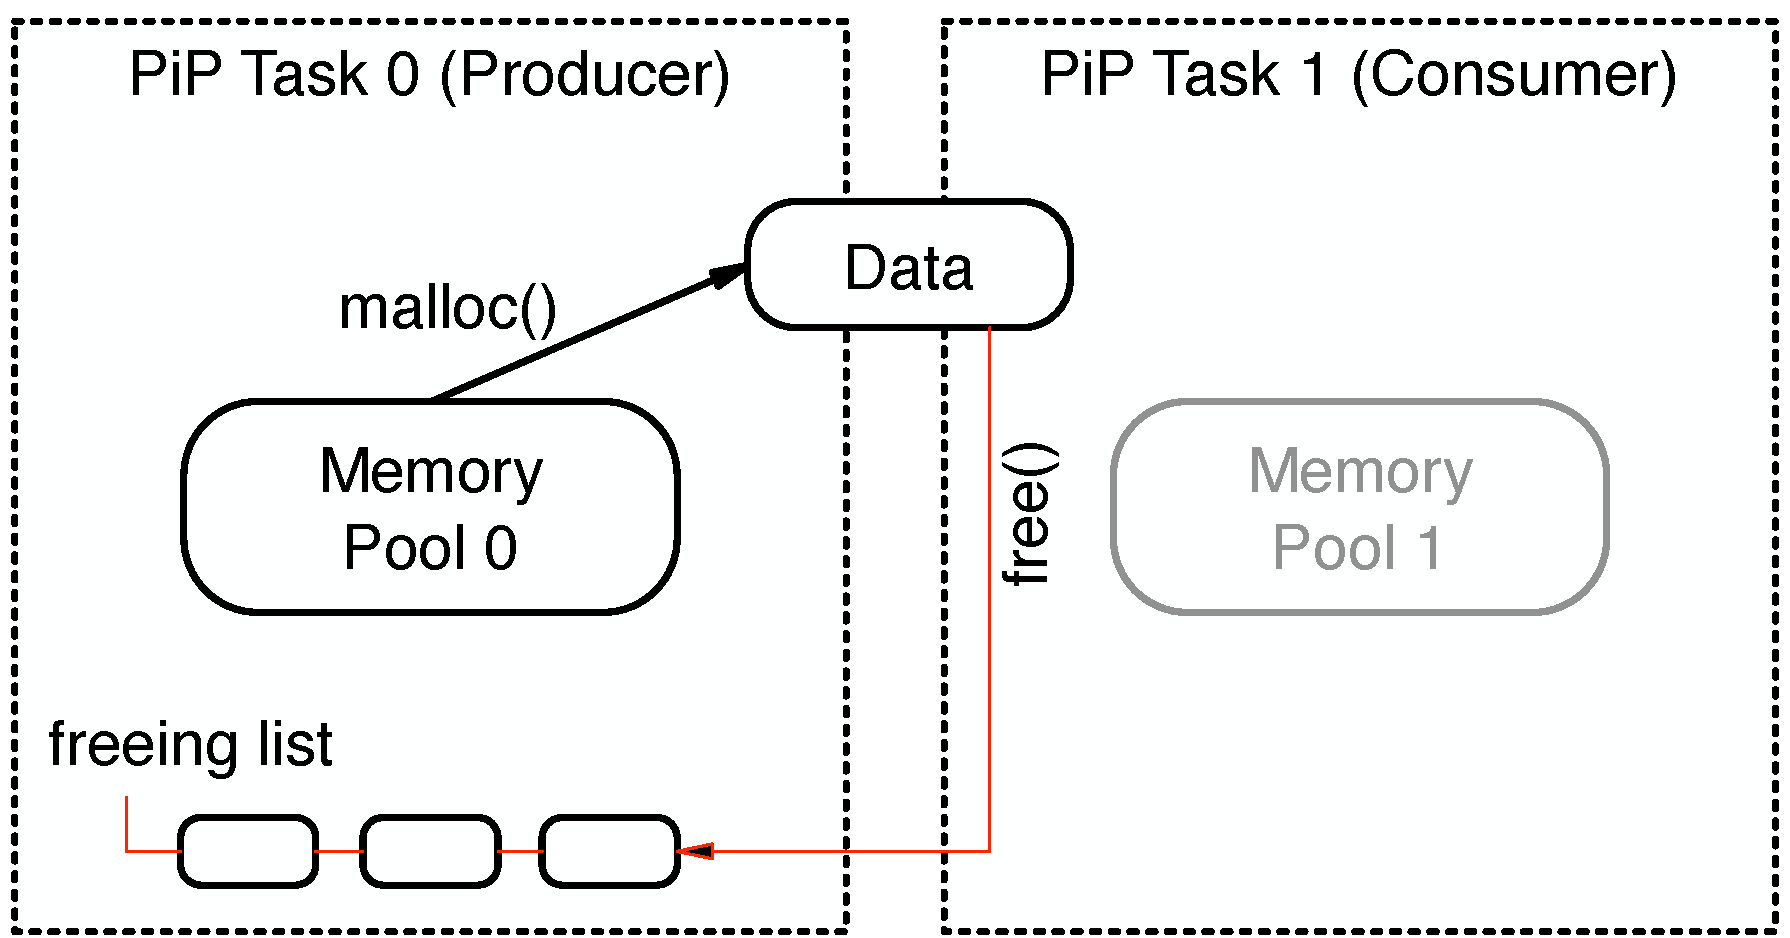
\includegraphics[width=0.7\columnwidth]{malloc/Figs/CrossMallocFree.pdf}
\caption{Cross-Malloc-Free with Freeing List}
\label{fig:cross-malloc-free}
\end{figure}

In order to address this, the PiP library wraps the {\tt malloc}
functions, as seen in Table 3.3. The \linuxfunc{malloc} wrapper
function embeds  the information about who allocated a memory
space. When this region is to be \linuxfunc{free}ed, the
\linuxfunc{free} wrapper function connects the region to the freeing 
list of the task allocating the region. When one of the wrapper
functions for {\tt malloc} is called, the regions in the freeing list
are really \linuxfunc{free}ed (Figure~\ref{fig:cross-malloc-free}). 


\section{{\tt XPMEM}}\label{sec:xpmem}

As described in Section~\ref{sec:shared-memory-myth}, {\tt
  XPMEM} is known to provide a shared memory model which is more
convenient that the POSIX shared memory. Again, the shared address
space which PiP provides includes the shared memory model which {\tt
  XPMEM} and POSIX shared memory provide. Thus, the same
functionalities of {\tt XPMEM} can also be implemented by using PiP.

The PiP library provides the same functions which are provides by {\tt
  XPMEM}.  Those who have programs using {\tt XPMEM} can easily switch
to using PiP.  By using PiP, there is no need of installing {\tt
  XPMEM} kernel module. Most importantly, {\tt XPMEM} functions
provided by PiP work much faster than those of {\tt XPMEM}. This is
because no system call involved to map memory segment of the other
process(es) in PiP. Indeed, most {\tt XPMEM} functions almost do
nothing since the other processes are already mapped from the
beginning in PiP. 


\chapter{PiP Internals}

\section{PiP Implementation and design choices}

\subsection{Spawning Tasks}\label{sec:spawn-details}

Prior to PiP version 2.4, the following steps were used to launch PiP
tasks:

\begin{enumerate}
\item The spawning program is loaded by calling \linuxfunc{dlmopen},
\item Glibc is initialized in the execution context of the loaded
  program,
\item Call \linuxfunc{clone} or \linuxfunc{pthread_create} (chosen
  by the \pipenv{PIP_MODE} environment setting) to spawn the PiP task,
\item The before hook is called if any, and finally
\item Jump into the starting function.
\end{enumerate}

Wrapper functions for the Glibc functions listed in
Table~\ref{tbl:pip-wrapper} were first introduced in PiP version
2.4. When developing these wrapper functions, I discovered that it is
nearly impossible to wrap the \linuxfunc{dlsym}.
A function wrapper is usually implemented as; 1) obtain the wrapping
function address by calling the \linuxfunc{dlsym} with the
\linuxdef{RTLD_NEXT} 
argument, 2) do the wrapping job before and/or after calling the
original function. The most of the Glibc \linuxfunc{malloc} routines has
the other weak symbols (\linuxfunc{malloc} and
\linuxfunc{__libc_malloc}, for example) and users can call the Glibc
\linuxfunc{malloc} routines without  
calling \linuxfunc{dlsym}. If there is no such weak symbol, we cannot
create a wrapper function for \linuxfunc{dlsym}. How can I
wrap a Glibc function without calling \linuxfunc{dlsym}?

I used another program, dubbed \pipterm{ldpip.so}, to resolve this
problem. thus to load the PiP library and user application. the method
for new spawning is described here;

\begin{enumerate}
\item Load \pipterm{ldpip.so} attached in the PiP library package by
  calling \linuxfunc{dlmopen} and jump into a function defined inside
  of it, 
\item The starting function of \pipterm{ldpip.so} initializes Glibc,
\item Obtain Glibc function addresses to wrap them later by the PiP
  library (\pipterm{libpip.so}),
\item Load \pipterm{libpip.so} by calling \linuxfunc{dlopen},
\item Load a user program by calling \linuxfunc{dlopen},
\item Call \linuxfunc{clone} or \linuxfunc{pthread_create} (chosen
  by the \pipenv{PIP_MODE} environment setting) to spawn the PiP task, 
\item Jump into a function inside of PiP library and initialize the
  PiP library, 
\item The before hook is called if any, and finally
\item Jump into the starting function in the user program.
\end{enumerate}

No wrapper functions are defined at the moment \pipterm{ldpip.so} is
loaded, making it simple to access the Glibc function addresses by
simply referencing them. The Glibc functions that need to be wrapped
are now wrapped using the function address table built by
\pipterm{ldpip.so} after loading \pipterm{libpip.so}.

It is necessary to run \linuxfunc{__ctype_init} with the execution
context (Section~\ref{sec:context}) of the launched PiP task in order
to initialize Glibc. In an earlier version of the PiP library, this
was accomplished by first obtaining the initialization function by
calling \linuxfunc{dlsym} on the loaded handle returned by
\linuxfunc{dlopen}, and then by executing the 
initialization function itself. The initialization process in the new
implementation consisted of calling the initialization method directly
from the ldpip.so file, where the execution context was the same as
that of the PiP task. So, things can go in an easier manner by
introducing PiP loader program (\pipterm{ldpip.so}).

\subsection{Calling {\tt clone()} System Call}\label{sec:clone}

PiP library uses a unique flag combination to call the
\linuxfunc{clone} system call, as explained in
Section~\ref{sec:spawn-details}. Since the \linuxfunc{clone} system
call takes a lot of inputs, some of which are difficult to implement,
I chose to wrap \linuxfunc{pthread_create} and \linuxfunc{clone} in
order to change only the flag setting.   

Wrapping the \linuxfunc{clone} system call is a challenge because it
is used by many libraries in addition to the PiP library (e.g.,
PThread library). When the PiP library calls the function, the flags
must be modified; however, when some other libraries call the same
method, the flags should not be changed. This is a circumstance that
cannot be handled by a straightforward function wrapping.

The test-and-set atomic instruction was used to construct a specific
locking mechanism in order to address this problem and prevent the
\linuxfunc{clone} system call from being invoked simultaneously from
the PiP library and from another source. The {\tt test-and-set}
instruction is used by the PiP library to lock when it is going to run
\linuxfunc{pthread_create} with the value of current thread ID (TID),
which ultimately invokes the \linuxfunc{clone} system call. The wrapper 
function of the \linuxfunc{clone} firstly tries to lock, but it fails
with value of the current TID, then it is the case of calling from the
PiP library. If the lock is successful, a different library will call
it. The original \linuxfunc{clone} is called with the altered flags in
the first scenario. In the latter scenario, the wrapper function call
calls \linuxfunc{clone} with the same input. Naturally, the lock is
released after the original \linuxfunc{clone} system call returns. 

\subsection{Execution Mode in Details}

The PiP's \pipterm{process mode} has two sub-modes:
\pipterm{process:preload} and \pipterm{process:pipclone}\footnote{In
  PiP implementation earlier than version 2.4, there was another mode 
\pipterm{process:got}. But this becomes obsolete in the newer
versions.}. Wrapping the \linuxfunc{clone} function mentioned above 
implements the \pipterm{process:preload} mode. The
\pipterm{process:pipclone} mode implements another
\linuxfunc{pthread_create}-like function in the \pipglibc\ (Section
3.2.2). If the PiP library is configured to use the \pipglibc,
\pipterm{process:pipclone} is taken; otherwise,
\pipterm{process:preload} is taken.  

\subsection{Name of PiP Tasks}\label{sec:proc-name}

The ability of the \pipcmd{pips} command (Section~\ref{sec:pips}) to
distinguish between PiP tasks and other customary processes and/or
threads may be unclear to certain readers. Each process and thread in
Linux has a name, which is visible in the COMMAND column of the top
command. The \linuxfunc{prctl} system call (in \pipterm{process mode})
or the \linuxfunc{pthread_ setname np} call (in \pipterm{pthread
  mode}) are used by the PiP library to set the command name. The 
first two characters of the name are used by the PiP library
(Table~\ref{tbl:name-1} and \ref{tbl:name-2})). 

\begin{table}[ht]
  \centering
  \caption{Command Name Setting (1st char.)}\label{tbl:name-1}
  \vspace{3mm}
  \begin{tabular}{c|c|l}
    \hline
    First char. & Distinction & \multicolumn{1}{c}{Note} \\
    \hline
    {\tt R} & PiP Root &  \\
    {\tt 0..9} & PiP Task & the least significant digit of \PIPID \\
    \hline
  \end{tabular}
\end{table}

\begin{table}[ht]
  \centering
  \caption{Command Name Setting (Second char.)}\label{tbl:name-2}
  \vspace{3mm}
  \begin{tabular}{c|lc|l}
    \hline
    2nd char. & Execution Mode & Abbreviation & Note\\
    \hline
    {\tt :} & \pipterm{process:preload} & {\tt L} & \\
    {\tt ;} & \pipterm{process:pipclone} & {\tt C} & \\
    {\tt .} & \pipterm{process:got} & {\tt G} & obsolete \\
    ${\tt \vert}$ & \pipterm{pthread} & {\tt T} & \\
    \hline
  \end{tabular}
\end{table}

PiP takes up the first two characters of the name, which can be up to
16 characters. The original command name is represented by the final
14 characters. The letters used by the pip-mode command
(Section~\ref{sec:pip-mode}) to specify the PiP execution mode are
shown in the abbreviation column of Table~\ref{tbl:name-2}. The
\pipcmd{pips} command may now identify the normal processes or threads
from the PiP roots and PiP tasks by using those first 2 characters of
the command name. 


\section{Remaining Issues}

\subsection{Recycling PiP Tasks}



\chapter{PiP Installation}

There are several ways to install PiP listed below;

\begin{itemize}
\item Building from source code
\item \pipcmd{pip-pip} command
\item Using \em{Spack}
\end{itemize}

It was scheduled to use RPM (yum)and Docker, but 
they are not available at the time of this writing.


\section{Building from Source Code}

Usually, building full PiP package consists of the following steps;

\begin{enumerate}
\item Building PiP-glibc (optional)\label{item:glibc}
\item Building PiP library
\item Building PiP-gdb (optional)\label{item:gdb}
\end{enumerate}

The \ref{item:glibc} and \ref{item:gdb} steps are optional, but
PiP-gdb requires PiP-glibc. So the possible combinations are;

\begin{itemize}
\item PiP library only
\item PiP-glibc and PiP library, and
\item PiP-glibc, PiP library and PiP-gdb.
\end{itemize}

Listing~\ref{out:build-source} shows a typical case of building full
set of PiP software package. 

\lstinputlisting[style=example, basicstyle=\footnotesize\tt,
  breaklines=true, 
  caption={Building from Source Code}, label=out:build-source]
                {install/examples/src-build.mout}


\section{\pipkw{pip-pip} command}

The procedure to install full set of PiP package might be cumbersome,
but installing PiP package by using the \pipcmd{pip-pip}
(\url{https://github.com/procinproc/PiP-pip}) command is much easier. 

\lstinputlisting[style=example, basicstyle=\footnotesize\tt,
  breaklines=true, 
  caption={PiP-pip installation example}, label=out:pip-pip]
                {install/examples/pip-pip.mout}


\section{Using Spack}

Spack is another installation tool
designed for the HPC software packages and PiP can also be installed
by using Spack. Listing~\ref{out:spack} shows the example of
installing PiP (including PiP-glibc)\footnote{Unfortunately, the
current version does not install PiP-gdb for some reason.}.

\lstinputlisting[style=example, basicstyle=\footnotesize\tt,
  breaklines=true, 
  caption={Spack installation example}, label=out:spack]
                {install/examples/spack.mout}



% Bibliography
\bibliography{pip}

\nocite{1-Hori18}%
\nocite{2-Hori20}%
\nocite{3-Ouyang20}%
\nocite{4-Ouyang21}%
\nocite{5-Hori22}%
\nocite{6-Ouyang22}%


%\appendix

\printindex

\end{document}
